\documentclass[12pt]{article}

\usepackage[letterpaper,total={6.5in,9.5in}]{geometry}                

\usepackage{amssymb,amsmath,graphicx, wasysym, url, setspace, moresize, float, lscape, afterpage}

\newcommand\blfootnote[1]{%
  \begingroup
  \renewcommand\thefootnote{}\footnote{#1}%
  \addtocounter{footnote}{-1}%
  \endgroup
}

\doublespacing

\graphicspath{{images/}}

\title{Heterogeneity in Returns to College Major}

\author{Oliver Titus}

\date{May 14, 2019}

\begin{document}
\maketitle

\abstract{This paper seeks to explore how one's college major impacts his or her wages. Using data from the American Community Survey, we explore 22 fields of bachelor degrees and test to see how they impact hourly wages using regression analysis. To see the true effect on wages, we control for race, marital status, employment type, as well as higher degrees. We find that the major category with the highest hourly wages is engineering and the major category with the lowest hourly wages is philosophy and religion.  We then focus the analysis on the difference in hourly wages by gender in each college major category. Findings suggest that hourly wages in each category differ by gender.}
\pagebreak
\section{Introduction}
\par If you want to obtain higher returns in the labor market, you would probably decide that you want to seek a college education. According to Becker (1975), education and training are the most important human capital investments and a high school and college education will greatly increase a person's income. The most important step to obtaining a college degree is choosing a field of study or a major. According to Altonji (2012), students choose their major based on several factors. One of those being preferences, which is based on the individuals favorite subjects in school. Another one being ability and preparation, which is how the individual is able to perform and master those subjects. The most important factor being the expectations of future earnings. According to a Georgetown University study done by Carnevale, et al 2015, about 35 percent of today's jobs require a Bachelor's degree or higher. Their study also finds that recent college graduates' annual wages vary from \$27,000 to \$50,000 depending on major choice.
 
\par In this paper, we seek to analyze the hourly wage returns to college major using regression analysis. We use data from the 2009 American Community Survey to determine how different fields of bachelor's degree affect hourly wage outcomes. To do this, we compare the hourly wages in each major category to those with a business degree since business majors were the most popular major in the data set. We include some controls in our analysis to the see the true effect. We include gender, race, marital status, as well as higher degree levels such as those with a masters degree, professional degree, or a PhD. We also run another regression that controls for the type of work individuals are doing such as profit, non-profit, unemployed and many other employment types.

\par We then shift our analysis to the hourly wage differences by gender. According to the U.S. Bureau of Labor Statistics, the women-to-men earnings ratio in 2009 was 80 percent, implying that women make about 20 percent less than men. Looking at woman's earnings by major, we do find that they are making less than men in most major categories, but not all of them. A Chow Test confirmed that the male and female slope coefficients for hourly wages are different.

\par  We will start off our analysis with a review of the literature as well as theory in section 2. In section 3, we will discuss the features of the ACS data set and then we will go over the methodology of how we obtained our results. Lastly, we will discuss the results in section 4 and move into some conclusions in section 5. Section 6 lists the works cited in this paper and section 7 shows figures and tables.

\section{Background}
\par A paper from the National Bureau of Economic Research by Altonji, et al (2012) used the same 2009 ACS data set used in this paper to determine the impacts of a higher education on labor market outcomes. Along with the ACS data, they pair characteristics associated with the different majors such as SAT scores, number of math and science courses, mean wages, and other characteristics using data from NCES B\&B. From this data, they note that "women are far more prevalent in education, and men in engineering business and economics" (21). They also observe that "...wages tend to be high for engineers and low for elementary education majors, suggesting that perhaps much of the wage differences between majors are due to differences in mathematical ability and high school course work" (21). They also analyze the 2009 ACS data using regression analysis to determine their findings.  Their regression included dummy variables for advanced degrees, a cubic for potential experience, and controls for race/ethnicity. Their main finding was consistent to that of the B\&B in that engineers have the highest returns and education majors have the lowest. Overall, they find that hourly wages vary greatly across college majors and that the variation is large enough for the tendency for men to choose higher paying college majors such as engineering to be an important factor in the gender gap in wages. They also conclude that a major part of the differences in returns is due to differences in the market value of tasks that require special skills and knowledge that certain majors develop.

\par  A Georgetown University study done by Carnevale, et al (2015) uses Census data to analyze wages for 137 college majors to detail the most popular college majors, the majors that are most likely to lead to an advanced degree, and the economic benefit of earning an advanced degree by an undergraduate major. Their analysis focuses on differences in median earnings for each major category. They find that the top paying college majors earn approximately \$3.4 million more than the lowest-paying majors over a lifetime. The highest paying majors are within the STEM fields whereas the lowest paying majors are in the fields of early childhood education, human services, and community organization. While they argue that the most lucrative majors are not the most popular, like Altonji (2012), they conclude that the economic value of college major plays a role in students' choice of major, but their academic preparation, interests and values are also important.

\par Another study done by Thomas Daymont (1984) used data from the National Studies of the High School Class of 1972 to analyze the gender gap in earnings from recent college graduates.  In their survey of literature, they find that researchers are unable to explain the male to female earnings difference which provides evidence that labor market discrimination is a factor to inequality in earnings. Daymont argues that differences in taste or preferences and preparation for many types of work measured before entering the labor market contributes to the earnings gap between males and females who are recent college graduates. They also use regression analysis to estimate the effects on earnings in relation to college major. Like Altonji (2012) and Carnevale (2015), they find that "the payoffs to traditionally male majors such as engineering and business are greater than the payoffs to traditionally female majors such as education."(418) In their analysis of the gender gap, they find that traditionally female majors like health or biology and education have greater returns for women whereas men have greater returns in traditionally male dominated fields such as engineering. They do find exceptions to this pattern however in that the coefficients were higher for women than men in business, science, math, or professional fields of study which they believe could be due to the possibility of improved opportunities for women in those fields. Daymont concludes that with elimination of labor market discrimination, there would still be a gap in male to female earnings since males and females have different preferences and ways of preparing for the labor market.

\par Becker (1975) found that education has a positive impact on an individuals wage even after controlling for the direct indirect costs of schooling, and after adjusting for better family backgrounds and greater abilities of more educated people. Altonji (2012) found that college major does matter for wages even after controlling for race and higher education levels. Carnevale (2015) said that there is some gender bias in the selection of major which yields a higher gender bias than estimated in standard occupation estimates. Therefore, this work will explore not only the heterogeneity in major payoff, but also the heterogeneity in both selection into major and returns to major by gender.

\section{Data}
\par To estimate the effects of hourly earnings on college major as well as difference in hourly earnings for each major by gender, we use 2009 American Community Survey data which is one of the data sources use in Altonji (2012). The ACS is a short-form questionnaire that contains questions regarding socioeconomic information. The survey asks many simple questions that include your name, sex, age, date of birth, race and ethnicity ("American Community Survey"). According to Table 1, the data surveys 1,270,870 individuals with ages ranging from 16 to 70 years. Figure 1 shows the distribution of ages. The individuals have between 1 to 24 years of education. A histogram for years of education is shown in Figure 2. We can see from Figure 2 that most people have a bachelor's degree (16 years of education) or higher. The mean income is approximately \$36,408.34 with a very high standard deviation of \$51,561.21 due to very strong outliers in the data. This can be seen by rightward skew of the income distribution in Figure 3.  

\par Table 2 shows a summary of the 17 majors that we test in this paper. These are more general categories of majors or meta-majors so to speak. For example, the business major category also includes Statistics and Economics majors. There some key observations that we can note from this table. We see that the most popular major is Business and least popular major is Transportation. The most popular male dominated major is Business being 57.2 percent male and the most popular female dominated major is Education being 76 percent female. The major with the highest average income is Engineering and major with the lowest average income is the Arts. This is also true for the female sample, however the male sample has the highest mean income with Science and lowest mean income with Health and Nutrition. We can also see that males have higher mean incomes in all major categories.

\par Figure 4 shows the male versus female income distribution for Business majors. We see that both the male and female distributions are right skewed. The female distribution is bimodal whereas the male distribution is unimodal. We can observe that plot for the male distribution lies rightward of the female distribution meaning that males have a higher mean income. This can also be observed in Table 2.

\par Figure 5 shows the male versus female income distribution for Education majors. Like the distribution for Business majors in Figure 4, we see that these distributions are right skewed. The male distribution is unimodal whereas the female distribution is bimodal. Like the Business major income distribution, we see a slight rightward shift of the male distribution plot, implying that males have a higher mean income than females despite Education majors being the most popular female dominated major at 76 percent female. This can also be observed in Table 2.     

\section{Empirical Model and Results}

\subsection{Empirical Model}
\par For this paper, our null hypothesis is that college major does not impact hourly wages. The alternative hypothesis would be that college major does impact hourly wages which is what this paper is testing for. This can be represented mathematically below:
\begin{align*}
H_0: \beta_{major} = 0 \\
H_a: \beta_{major} \neq 0
\end{align*}
Equation (1) is the main regression specification used in this paper to test for college major wage heterogeneity:
\begin{equation}
\ln(Y_i) = \beta_0 + \beta_1 X_i + \beta_2 E_i + \beta_3 R_i + \beta_4 F_i + \beta_5 M_i + \beta_6A_i + \beta_7A_i^2 + \epsilon_i
\end{equation}
\begin{itemize}
\item $Y_i$ is the hourly wage.
\item $X_i$ is the set of major dummies with Business Majors being set as the base.
\item $E_i$ is higher degree levels including masters, professional degree, and PhD.
\item $R_i$ is the set of races.
\item $F_i$ is a female dummy variable.
\item $M_i$ is dummy variable that denotes marital status.
\item $A_i$ is age.
\item $\epsilon_i$ is other factors not accounted for.
\end{itemize} 
We also control for the individual's type of work. Work types from the ACS data includes private sector for profit, private sector not for profit, local, state, or federal government, self-employed in own non-incorporated business, self-employed in own incorporated business, working without pay in family business, as well as unemployed. Equation (2) is regression specification used to control for work type:
\begin{equation}
\ln(Y_i) = \beta_0 + \beta_1 X_i + \beta_2 E_i + \beta_3 R_i + \beta_4 F_i + \beta_5 M_i + \beta_6A_i + \beta_7A_i^2 + \beta_8W_i + \beta_9X_{bi}*W_i + \beta_{10}X_{ei}*W_i + \epsilon_i
\end{equation}
This is similar to equation (1), however we add the following controls:
\begin{itemize}
\item $W_i$ controls for work-type with non-profit work being set as the benchmark.
\item $X_{bi}*W_i$ is an interaction that controls for business majors and their work-types.
\item $X_{ei}*W_i$ is an interaction that controls for education majors and their work-types.
\end{itemize}
We also test for the differences in wage for select college majors by gender. To test for this, we use equation (3):
\begin{equation}
\ln(Y_i) = \beta_0 + \beta_1F_i + \beta_2X_i + \beta_3X_i*F_i + \epsilon_i
\end{equation}
Here we remove all the controls because all we want to see how much more or less women are making in their majors compared to men on average. We add the following interaction term:
\begin{itemize}
\item $X_i*F_i$
\end{itemize} 
This is an interaction with the female dummy and major. The coefficient $\beta_3$ will give us the percentage hourly wage difference between males and females for each major.
\subsection{Results}
\par We test the hypothesis that education, major, and gender matter in determining wages. Our results are displayed in Table 3 and Table 4. Table 3 shows results based on equations (1) and (2). Table 3 shows hourly wage differences across each major with Business majors being set as the benchmark. This is why Business majors are omitted from this table. A regression was run for the full sample which is based on equation (1) as well as the full sample with the work-type controls shown in equation (2). We also ran regressions based on equation (1) with the male sample as well as the female sample. One thing to note about the regression for the male and female sample is that the female dummy is removed; otherwise, this would cause multicollinearity. From Table 3, we can see that there are significant differences in log hourly wages across the majors. Since we are looking at log hourly wages, Table 3 shows percentage difference in hourly wage compared to Business majors. For example, Mathematics majors in the full sample on average make 6.2 percent more in hourly wages compared to Business majors. It is also noteworthy that those without a bachelor's degree in the full sample make 52.2 percent less in hourly wages compared to Business majors. In the full sample with the work-type controls they make 42.7 percent less on average. The males make 50.7 percent less compared to male Business majors on average. The females make 52.6 percent less compared to female Business majors on average. 

\par There are some key observations that we can see in Table 3. We see that across all samples, engineering majors have the highest returns in hourly wages. In the full sample, they make 17.8 percent more in hourly wages compared to Business majors on average. In the full sample with work-type controls, they make 26.6 percent more. In the male sample, engineering males make 16.6 percent more on average in hourly wages compared males who are Business majors. Females with an engineering major make 23.3 percent more in hourly wages compared to female business majors. The lowest paying major is philosophy and religion which can be seen across all the samples. In the full sample they make 47.4 percent less on average in hourly wages compared to business majors. In the full sample with the work-type controls, they make 36.2 percent less on average. In the male sample, they make 52.8 percent less on average compared to male business majors on average. The female philosophy and religion majors make 34.2 percent less in hourly earnings compared to female business majors on average.

\par There are few other things to note about Table 3. We see that there are a few results that are insignificant. Most of the coefficients for transportation majors are insignificant except when we control for work-type. This is likely due to the smaller sample size of transportation majors. We also see that the education majors in the full sample with work type controls are omitted. This is likely due to the education dummy being highly correlated with the interaction of education majors and state government employees. This collinearity is likely due to the fact that teachers are considered state government employees. 

\par Table 4 shows us the female percentage hourly wage difference across select majors. This table is based off of equation (3). For example, we see that female Mathematics majors make 6.21 percent less hourly wages compared to male Mathematics majors on average. We see that some of the coefficients are negative, suggesting that women are making less than men with these majors. Some of this could be due to labor market discrimination, however, we did not analyze what jobs these women are choosing. However, we did perform a Chow Test. 

\par A Chow Test is a special type of F-test that determines whether or not the slope coefficients between two groups are the same (Wooldridge 2013). In this case, the Chow Test reports whether wage determinants, such as major, differ significantly by gender. The test returned a large F-statistic of 2996.41 which gives a P-vale less than 0.01. This implies that hourly wages are different for men in women in each major category with high statistical significance. This difference in slopes across majors for males and females could be due to women choosing jobs that are less lucrative or women are not promoting to the same rank as men with similar occupations. We can also see that the coefficients are positive and significant for computers, education, philosophy and religion, as well as art majors. This is likely due to improved opportunities for women in these fields like Daymont (1984) mentions. 

\par These findings are quite similar to other researchers have found in the literature. While Altonji (2012) found that engineers have the highest returns, they found that education majors had the lowest returns. Altonji analyzed 171 specific college majors in their study. Here, those majors are contained in 22 different categories which could be a reason why we reach a slightly different conclusion in that philosophy and religion majors are getting the lowest returns. Our results are also consistent with Carnevale (2015) in that the highest paying majors are STEM fields whereas the lowest paying are humanities based majors. Daymont (1984), also found that the returns to education majors are lower than the payoffs to engineering and business majors which is also shown in our results.
 
\section{Conclusion}
\par In summary, we found that engineering majors have the highest hourly wage returns on average and philosophy and religion majors have the lowest hourly wage returns on average. This result is true for the full sample with and without work-type controls, as well as the male and female samples. We also found that female hourly wages are lower than male hourly wages in many of the majors. However, we did find that females with an art, education, computer, or philosophy and religion major make more hourly earnings than their male counterparts. The Chow Test confirmed that hourly wages are different for men and women in each major category.  

\par There are some limitations to this study that we want to recognize. The coefficients seen in the results might not represent the true effect of hourly wage differences by major for several reasons. One issue that we want to point out is omitted variable bias. The ACS data set did not include any socioeconomic background indicators like parental income or occupation. The lack of controlling for family background is likely making these coefficients biased. There were also some strong outliers in the hourly wage data which is likely making the effect on hourly wages based on college major larger than it actually is.

\par In future work, it would be interesting to see what percentage of individuals with a certain college major have an occupation that relates to their major. It would also be useful to control for occupation which we could not do in this study due to limitations with STATA/IC. It would also be useful in future work to analyze why women make less than men with certain majors by looking at the occupations that women are choosing as well what position they hold in that occupation compared to men.

\section{References}

\begin{enumerate}
\item Altonji, Joseph G., et al. “Heterogeneity in Human Capital Investments: High School Curriculum, College Major, and Careers.” Annual Reviews, \\ www.annualreviews.org/doi/abs/10.1146/annurev-economics-080511-110908.

\item Becker, Gary S. Human Capital: a Theoretical and Empirical Analysis, with Special Reference to Education. Columbia Univ. Press, 1975.

\item Bureau of Labor Statistics, U.S. Department of Labor, The Economics Daily, Women’s-to-men’s earnings ratio by age, 2009 on the Internet at \\ https://www.bls.gov/opub/ted/2010/ted\_20100708.htm (visited May 07, 2019).

\item Carnevale, Anthony P., et al. “The Economic Value of College Majors.” CEW Georgetown, 12 June 2018, cew.georgetown.edu/cew-reports/valueofcollegemajors/ 

\item Daymont Thomas N., et al. “Job preferences, college major, and the gender gap in earnings.” 
The Journal of Human Resources. Vol. 19, No. 3. 1984. pp. 408-428

\item Gauthier, Jason. “American Community Survey - History - U.S. Census Bureau.” American Community Survey - History - U.S. Census Bureau, \\
www.census.gov/history/www/programs/demographic/american\_community\_survey.html.

\item Wooldridge, Jeffrey M. Introductory Econometrics: a Modern Approach. South-Western Cengage Learning, 2013.
\end{enumerate}

\section{Appendix}

\subsection{Figures}

\begin{figure}[H]
\centering
\caption{Age Distribution}
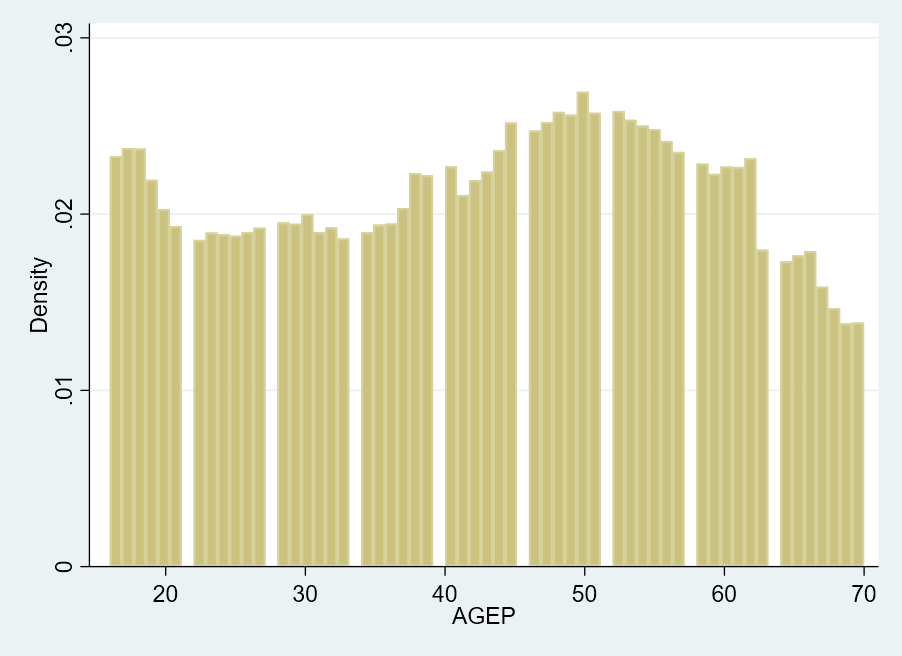
\includegraphics[scale=0.35]{age.png}
\end{figure}
\begin{center}
\footnotesize The horizontal axis here is age.
\end{center}
\begin{figure}[H]
\centering
\caption{Years of Education Distribution}
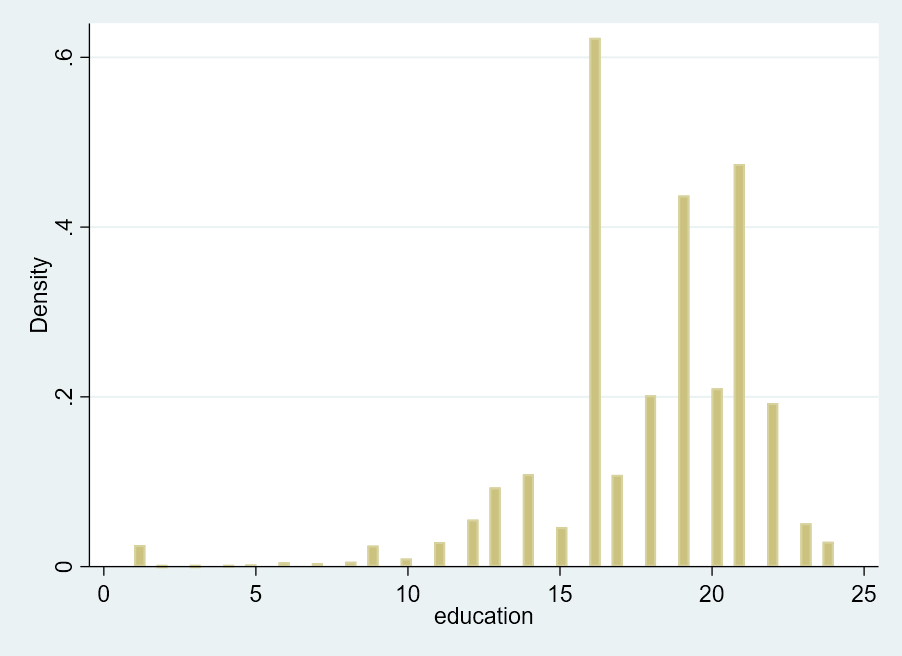
\includegraphics[scale=0.35]{eduhist.png}
\end{figure}

\begin{figure}[H]
\centering
\caption{Income Distribution}
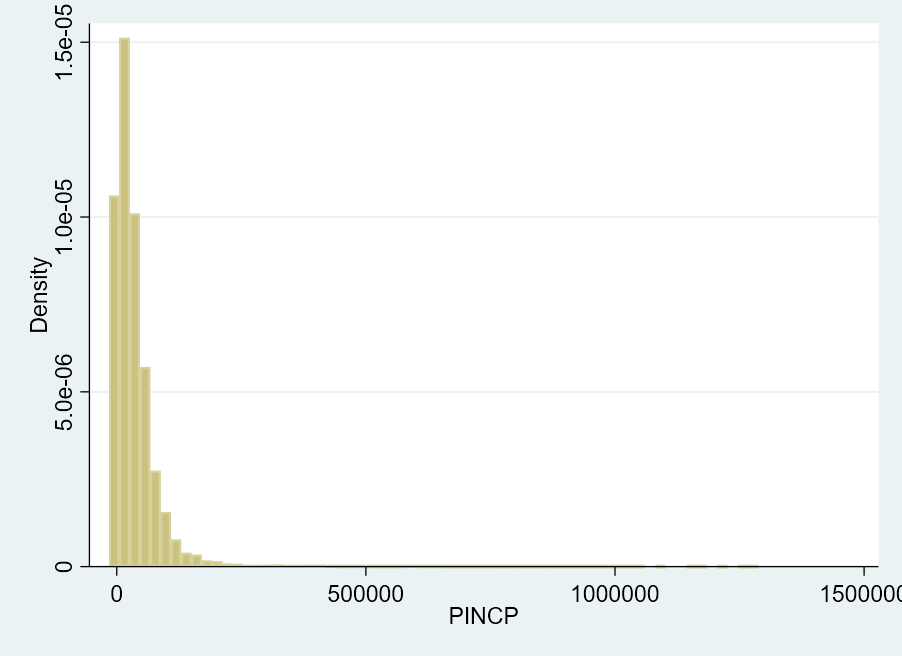
\includegraphics[scale=0.35]{income.png}
\end{figure}
\begin{center}
\footnotesize The horizontal axis here is income.
\end{center}
\begin{figure}[H]
\centering
\caption{Male vs. Female Income Dispersion for Business Majors}
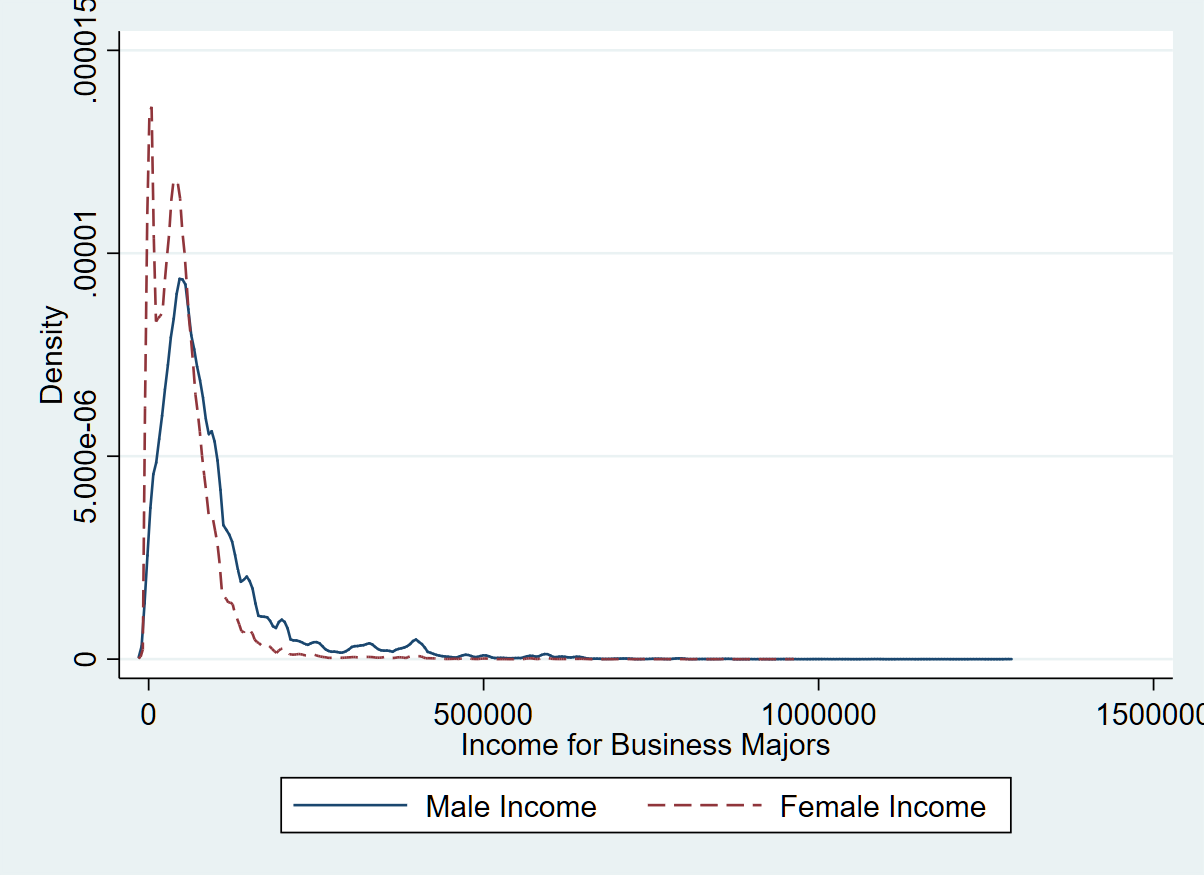
\includegraphics[scale=0.27]{business.png}
\end{figure}

\begin{figure}[H]
\centering
\caption{Male vs. Female Income Dispersion for Education Majors}
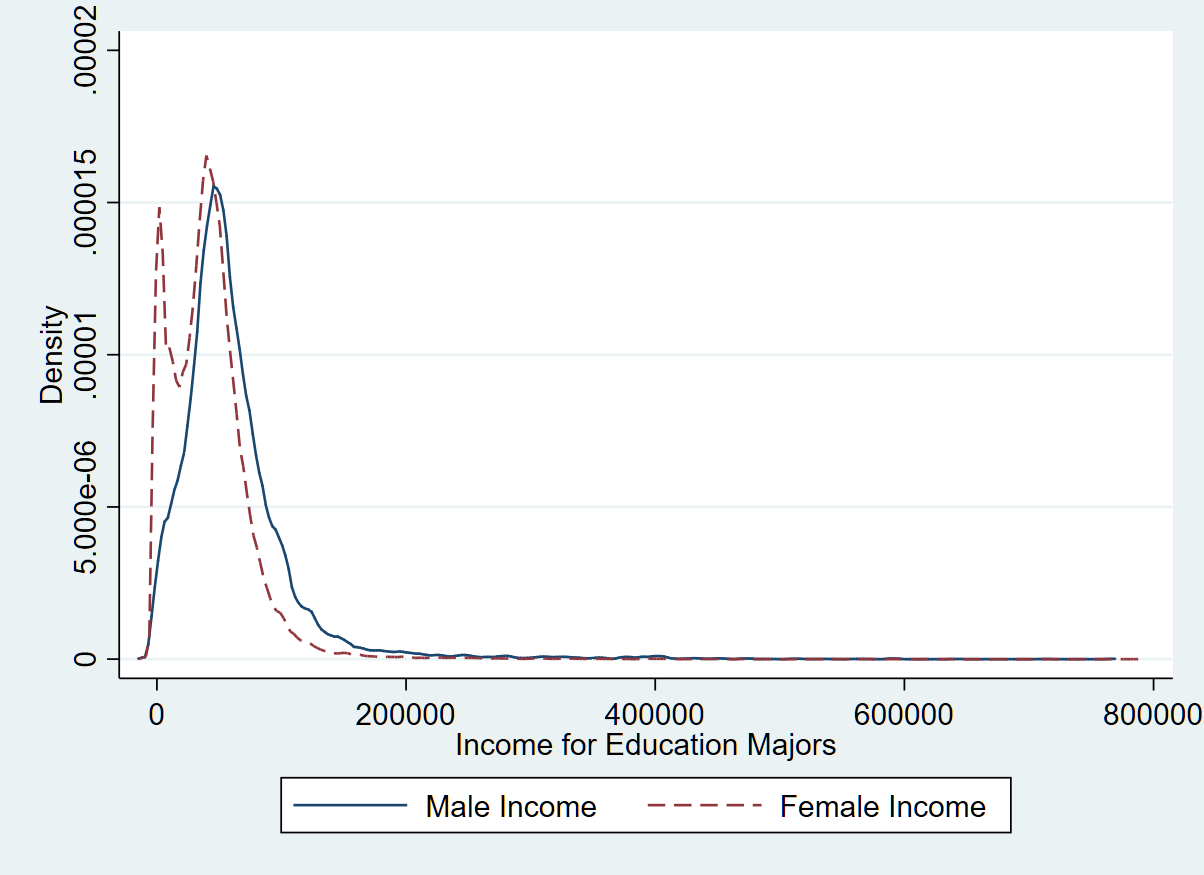
\includegraphics[scale=0.27]{education.png}
\end{figure}

\subsection{Tables}
\begin{center}
\begin{table}[H]
\centering
\caption{Descriptive Statistics}
\begin{tabular}{|c | c c c c|}
\hline
\textbf{Variable} & \textbf{Mean} & \textbf{Std. Dev.} & \textbf{Min} & \textbf{Max} \\
\hline
Age &   42.862   &  15.293     &    16    &     70\\
Education (years) &   17.852  &  3.522   &       1  &       24 \\
Income (\$) &    36408.34  &  51561.21  &   0  &  1288000 \\
Annual Hours Worked &  1778.78  &  793.21     &    7    &   5049 \\
Hourly Wage (\$)   &  22.49  &  78.2   &       0  & 53571.43 \\
\hline
\end{tabular} \\
\begin{flushleft}
\footnotesize \textbf{n}=1270870
\end{flushleft}
\end{table}
\end{center}

\begin{landscape}
\begin{center}
\begin{table}[htbp]
\centering
\caption{Summary of Majors}
\begin{tabular}{|c | c c c c c |}
\hline
\textbf{Major} & \textbf{Frequency} & \textbf{Mean Income} & \textbf{Male Mean Income} & \textbf{Female Mean Income} & \textbf{\% Female} \\
\hline
N/A (less than college) & 1482644 & 25450.57 & 31760.58 & 19359.95 & 50.8\\
Agriculture &  9702 & 62481.52 & 72682.16 & 40690.92 & 31.9\\
Architecture &  3795 & 70561.38 & 82251.73 & 44579.04 & 30.9\\
Other Social Science & 69987 & 72581.21 & 94403.95 & 48836.69 & 47.9\\
Communications & 19749 & 54973.29 & 70323.80 & 44128.22 & 58.6\\
Computers & 14111 & 75615.37 & 83333.03 & 57583.66 & 29.9\\
Arts & 20641 & 44023.49 & 56310.76 & 36900.29 & 63.3\\
Education & 73398 & 46043.66 & 61501.54 & 41167.26 & 76\\
Engineering & 39376 & 94432.54 & 99884.08 & 61831.76 & 14.3\\
Liberal Arts & 38337 & 54426.15 & 78906.17 & 43662.41 & 69.5\\
Science & 41861 & 85256.39 & 108372.21 & 56228.25 & 44.3\\
Mathematics & 8278 & 82996.05 & 100341.93 & 59075.04 & 42\\
Health and Nutrition & 5149 & 45932.28 & 55910 & 38671.22 & 57.8\\
Philosophy and Religion & 7035 & 54325.06 & 61772.93 & 37840.55 & 31.1\\
Psychology & 24747 & 54190.59 & 79821.63 & 42844.80 & 69.3\\
Business & 104022 & 74961.10 & 93695.97 & 50910.04 & 43.8\\
Transportation & 1226 & 78031.10 & 81452.02 & 46207.85 & 9.7\\
Medical/Health Services & 34501 & 61077.82 & 96893.50 & 54049.98 & 83.6\\
\hline
\end{tabular}
\end{table}
\end{center}
\end{landscape}
\begin{landscape}
\begin{center}
\begin{table}[htbp]
\centering
\caption{Wage Heterogeneity by Major}
\begin{tabular}{| c | c c  c  c |}
\hline
\textbf{Major} & \textbf{Full Sample (\%)} & \textbf{Full Sample with} & \textbf{Males Only (\%)} & \textbf{Females Only (\%)} \\
 & & \textbf{Work Type Controls (\%)} & & \\
\hline
N/A (less than college) & -52.2*** & -42.7*** & -50.7*** & -52.6***\\
Agriculture & -27.3*** & -17.2*** & -30.2*** & -22.8***\\
Architecture &  -4*** & 6.6** & -4.8*** & -3.2\\
Other Social Science & -9.9*** & -0.1 & -8.8*** & -11.1***\\
Communications & -12.3*** & -2 & -16.4*** & -8.4\\
Computers & 12.8*** & 22.1*** & 12.9*** & 14.1***\\
Arts & -28.3*** & -16.8*** & -31.5*** & -25.2***\\
Education & -26.7*** & 0 (omitted) & -35.5*** & -22***\\
Engineering & 17.8*** & 26.6*** & 16.6*** & 23.3***\\
Liberal Arts & -18.8*** & -8.2*** & -20.2*** & -17.2***\\
Science & -4.2*** & 5.5** & -3.4*** & -5.4***\\
Mathematics & 6.2*** & 15.7*** & 7.8*** & 4.9***\\
Health and Nutrition & -24.3*** & -13.6*** & -31.7*** & -17.6***\\
Philosophy and Religion & -47.4*** & -36.2*** & -52.8*** & -34.2***\\
Psychology & -18.4*** & -7.8*** & -20.4*** & -17.1***\\
Transportation & 0.7 & 7.4** & -0.5 & 1.8\\
Medical/Health Services & 10.3*** & 20.3*** & 4.8*** & 13.2***\\
\hline
\end{tabular}
\end{table}
\end{center}
\blfootnote{***p $<$ 0.01 **p $<$ 0.05 *p $<$ 0.1
\\ \textbf{Note:} female dummy had a coefficient of -0.21 in the full sample with and without the work type controls, implying that females make 21\% less than men on average. Controls such as PhD, masters, professional degree, marital status, age, as well as a quadratic for age are not reported in this table. Standard errors are also not reported due to most of the major dummy coefficients being highly statistically significant. }
\end{landscape}
\begin{center}
\begin{table}[H]
\centering
\caption{Gender Wage Heterogeneity by Major}
\begin{tabular}{|c |c|}
\hline
\textbf{Major} & \textbf{Female Hourly Wage Difference (\%)} \\
\hline
Business & -6.31*** \\
Computers & 3.82** \\
Mathematics & -6.21*** \\
Education & 9.15*** \\
Engineering & 0.62 \\
Liberal Arts & -1.98** \\
Medical/Health Services & -0.93 \\
Philosophy and Religion & 11.03*** \\
Psychology & -4.70*** \\
Science & -13.76*** \\
Art & 5.31*** \\
\hline
\end{tabular}
\end{table}
\blfootnote{***p $<$ 0.01 **p $<$ 0.05 *p $<$ 0.1 \\ \textbf{Note:} female dummy had a coefficient of -0.22 implying that females make 22\% less than men on average. Only the coefficients are reported and standard errors/t-statistics are omitted.}
\end{center}

\end{document}

